
%=========================================================
\section{Módulos del sistema}

    El sistema se encuentra organizado por módulos con la finalidad de agrupar y administrar de mejor manera los requerimientos funcionales del sistema. Dividir el sistema en módulos permite visualizar e identificar rápidamente aquellos aspectos funcionales que pueden tratarse conjuntamente. \\
%
%    La figura \ref{fig:ModulosPAEAR} muestra los módulos propuestos de manera inicial para el \saear. Cada uno de estos módulos agrupan los casos de uso que poseen funcionalidad similar o que trabajan en conjunto para alcanzar un aspecto funcional del sistema. Cada uno de los módulos que se muestran en la figura se describen a continuación:

%    \begin{figure}[h!]
%	\begin{center}
	     % \fbox{\includegraphics[width=\textwidth]{images/modulos.jpg}}
%	\caption{Módulos del \saear.}
%	\label{fig:ModulosPAEAR}
%	\end{center}
%    \end{figure}

    \begin{itemize}
    \item {\bf Módulo Academias:} Agrupa los casos de uso que tienen que ver con la gestión de las academias existentes en la Escuela Superior de Cómputo.
	
	\item {\bf Módulo Infraestructura:} Agrupa los casos de uso que tienen que ver con la gestión de la infraestructura, la cual incluye la gestión de los edificios y espacios de la Escuela Superior de Cómputo.

	\item {\bf Módulo Oferta Educativa:} Agrupa los casos de uso que permiten la gestión de la oferta educativa de la Escuela Superior de Cómputo, incluyendo la gestión de los planes de estudio y las unidades de aprendizaje.
    
	\item {\bf Módulo Profesores:} Agrupa los casos de uso que permiten la gestión de los profesores que imparten las unidades de aprendizaje en la Escuela Superior de Cómputo.	

	\item {\bf Módulo Configuración General:} Agrupa los casos de uso que permiten crear un proyecto para generar horarios y las restricciones que tendrán estos. 
	
	\end{itemize}

	

%=========================================================
\section{Actores del Sistema} \label{sec:Comportamiento:ActoresSistema}

Los actores son los perfiles asociados a las diversas áreas y/u organizaciones que intervienen en el proceso. Se han identificado los actores de acuerdo a las actividades y responsabilidades dentro del TLAMATINIME: Timetabling Problem, Prototipo de Optimización de Horarios en la ESCOM, los cuales se muestran en la figura \ref{fig:perfiles} y se describen a continuación.

%    \begin{figure}[h!]
%      \begin{center}
%	  \includegraphics[width=0.6\textwidth]{images/actores/Actores.png}
%      \caption{Perfiles identificados.}
%      \label{fig:perfilesPAEAR}
%      \end{center}
%    \end{figure}

%SUBDIRECTOR ACADÉMICO
\cdtLabel{Actor:SA}{}
\begin{actor}{Subdirector Académico}{Es la persona encargada de la planificación de la Estructura Educativa en la Escuela Superior de Cómputo.}

	\item[Área:] Subdirección Académica.
	\item[Responsabilidades:] \hspace{1pt}
		\begin{itemize}
		    \item Registrar, modificar y eliminar las academias existentes en la Escuela Superior de Cómputo.
		    
		   	\item Registrar, modificar, eliminar y consultar la infraestructura para la Escuela Superior de Cómputo, esto incluye a edificios y espacios.
		   	
		   	\item Registrar, modificar, eliminar y consultar los planes de estudio vigentes en la Escuela Superior de Cómputo.
		   	
		   	\item Registrar, modificar, eliminar y consultar las unidades de aprendizaje ofertadas para el plan de estudio vigente. 
		   	
		   	\item Registrar, modificar, eliminar y consultar a los profesores que son los encargados de impartir las unidades de aprendizaje ofertadas en la Escuela Superior de Cómputo. 
		   	
			\item Registrar, modificar, eliminar y consultar los proyectos para generar la Estructura Educativa.
			
			\item Ejecutar el algoritmo encargado de hacer los horarios.
			
		 \end{itemize}
	\item[Perfil:] \hspace{1pt}
		\begin{itemize}
		    \item Persona que conoce el proceso de la Estructura Educativa.
	    \end{itemize}
	\item[Cantidad:] Uno por la ESCOM
\end{actor}


%CAPTURISTA
\cdtLabel{Actor:C}{}
\begin{actor}{Capturista}{Es la persona encargada de capturar la información necesaria en el sistema, para generar la Estructura Educativa de la Escuela Superior de Cómputo.}
	
	\item[Área:] No existente.
	\item[Responsabilidades:] \hspace{1pt}
	\begin{itemize}
		\item Registrar, modificar y eliminar las academias existentes en la Escuela Superior de Cómputo.
		
		\item Registrar, modificar, eliminar y consultar la infraestructura para la Escuela Superior de Cómputo, esto incluye a edificios y espacios.
		
		\item Registrar, modificar, eliminar y consultar los planes de estudio vigentes en la Escuela Superior de Cómputo.
		
		\item Registrar, modificar, eliminar y consultar las unidades de aprendizaje ofertadas para el plan de estudio vigente. 
		
		\item Registrar, modificar, eliminar y consultar a los profesores que son los encargados de impartir las unidades de aprendizaje ofertadas en la Escuela Superior de Cómputo. 
		
	\end{itemize}
	\item[Perfil:] \hspace{1pt}
	\begin{itemize}
		\item Persona que captura información en el sistema.
	\end{itemize}
	\item[Cantidad:] Tres por la ESCOM.
\end{actor}


%JEFE DE DEPARTAMENTO
\cdtLabel{Actor:JD}{}
\begin{actor}{Jefe de Departamento}{Es la persona encargada de gestionar parte del proyecto para generar la Estructura Educativa de la Escuela Superior de Cómputo.}
	
	\item[Área:] Varias.
	\item[Responsabilidades:] \hspace{1pt}
	\begin{itemize}
		\item Registrar, modificar y consultar los proyectos para generar la Estructura Educativa.
		
		\item Ejecutar el algoritmo encargado de hacer los horarios.
		
	\end{itemize}
	\item[Perfil:] \hspace{1pt}
	\begin{itemize}
		\item Persona que realiza parte de la creación del proyecto para generar la Estructura Educativa en el sistema.
	\end{itemize}
	\item[Cantidad:] El jefe de cada uno de los departamentos de la ESCOM.
\end{actor}


\newpage 
%%====================================================================================Academias

\section{Casos de Uso del módulo de Academias}

La figura \ref{fig:casosUso:gestionarAcademias} muestra los casos de uso que integran la funcionalidad del módulo de gestionar academias, el cual conlleva el registro, edición, modificación tanto de las mismas.
\begin{figure}[htpb!]
	\begin{center}
		\fbox{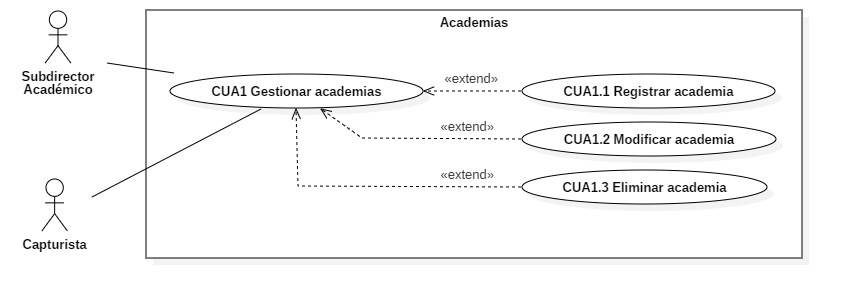
\includegraphics[scale=0.2]{ModeloComportamiento/Academias/imagenes/Academias}}
		\caption{Diagrama de casos de uso del módulo Academias \label{fig:casosUso:gestionarAcademias}}
	\end{center}
\end{figure}

%%====================================================================================Infraestructura

\section{Casos de Uso del módulo de Infraestructura}

La figura \ref{fig:casosUso:gestionarInfraestructura} muestra los casos de uso que integran la funcionalidad del módulo de gestionar infraestructura, el cual conlleva el registro, modificación, consulta, eliminación de los edificios y el registro, modificación, consulta, eliminación de los espacios dentro de un edificio.
\begin{figure}[htpb!]
	\begin{center}
		\fbox{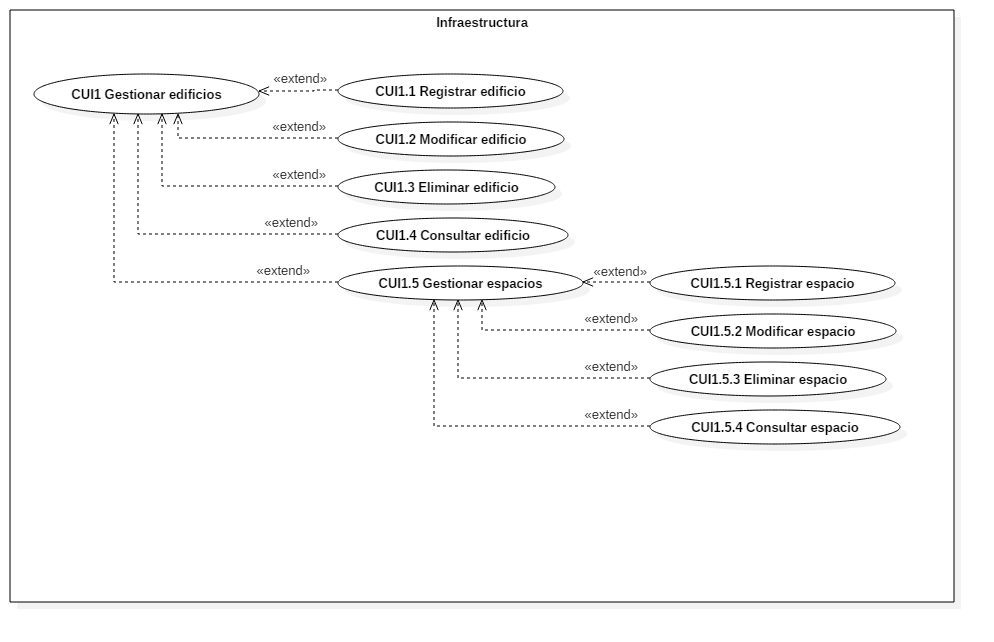
\includegraphics[scale=0.2]{ModeloComportamiento/Infraestructura/imagenes/Infraestructura}}
		\caption{Diagrama de casos de uso del módulo Infraestructura \label{fig:casosUso:gestionarInfraestructura}}
	\end{center}
\end{figure}

%%====================================================================================Infraestructura

\section{Casos de Uso del módulo de Oferta Educativa}

La figura \ref{fig:casosUso:gestionarOfertaEducativa} muestra los casos de uso que integran la funcionalidad del módulo de gestionar oferta educativa, el cual conlleva el registro, modificación, consulta, eliminación de los planes de estudio y el registro, modificación, consulta, eliminación de las unidades de aprendizaje ofertadas en dicho plan de estudio.
\begin{figure}[htpb!]
	\begin{center}
		\fbox{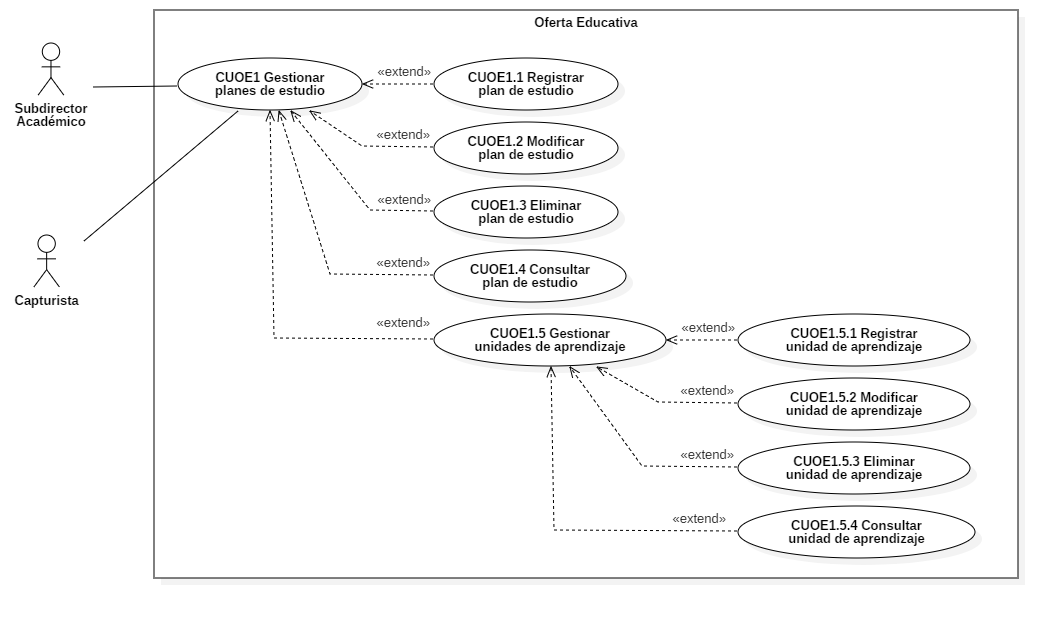
\includegraphics[scale=0.2]{ModeloComportamiento/OfertaEducativa/imagenes/OfertaEducativa}}
		\caption{Diagrama de casos de uso del módulo Oferta Educativa \label{fig:casosUso:gestionarOfertaEducativa}}
	\end{center}
\end{figure}
